\documentclass[pdf,11pt]{beamer}
\mode<presentation>{\usetheme{CambridgeUS} \usecolortheme{rose}
\useinnertheme{circles} % or rectangles, rounded
%\useoutertheme{infolines}
}

\usepackage{mathtools}
\usepackage{tikz}
\usetikzlibrary{arrows}

\usepackage[utf8]{inputenc}
\usepackage[english]{babel}
\usepackage{amsmath}
\usepackage{amsfonts}
\usepackage{amssymb}
\usepackage{graphicx}


\DeclareMathOperator*{\argmax}{arg\!\max}

\graphicspath{{./images/}}

\author[Pratyaksh \and Paramdeep]{Pratyaksh Sharma \and Paramdeep Singh}

\title[Keyword Querying]{Entity Relationship Keyword Querying \\ on Knowledge Graph}

%\institute{
\includegraphics[height=0.8cm]{iitb_logo.jpg}\vspace{220pt}}

\titlegraphic{
\includegraphics[height=50pt]{iitb_logo.jpg}}

\setbeamercovered{transparent}
%\setbeamertemplate{navigation symbols}{}
%\logo{}
\date{26 November 2015}
%\institute{IIT Bombay}

\begin{document}

\begin{frame}
  \titlepage
\end{frame}

%---------------------%
\begin{frame}
  \frametitle{Outline}
    \tableofcontents[hideallsubsections]
\end{frame}

%---------------------%
\section{Motivation}
\begin{frame}
  \frametitle{Outline}
    \tableofcontents[currentsection,hideallsubsections]
\end{frame}


%---------------------%
\begin{frame}{Motivation}
\begin{itemize}
\item Several large repositories of structured data available
  \begin{itemize}
  \item Freebase for example has over 1 billion facts
  \end{itemize}
\item Structured query languages (like SPARQL) are not usable by users who do not have sufficient schema knowledge
\item Current approaches towards keyword querying do not fare well on complex queries
\end{itemize}

\end{frame}

%-------------------%

\subsection{Problem Statement}
\begin{frame}{Problem Statement}

\begin{block}{Problem Statement}
Enable evaluation of complex keyword queries on large structured knowledge bases.
\end{block}

\end{frame}


%-------------------%
\section{Background}

\begin{frame}
  \tableofcontents[currentsection,hideallsubsections]
\end{frame}


%-------------------------%
\subsection{RDF}
\begin{frame}{RDF}
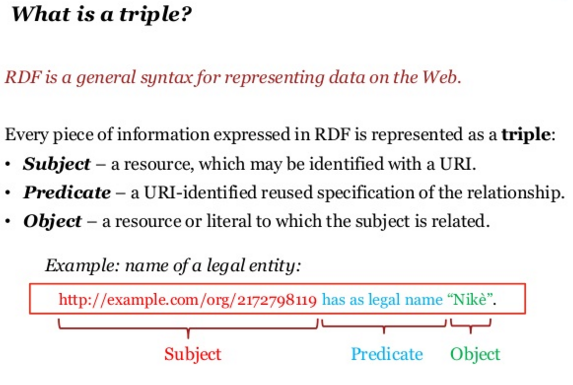
\includegraphics[height=8cm]{./1.PNG}
\end{frame}

\begin{frame}{RDF}
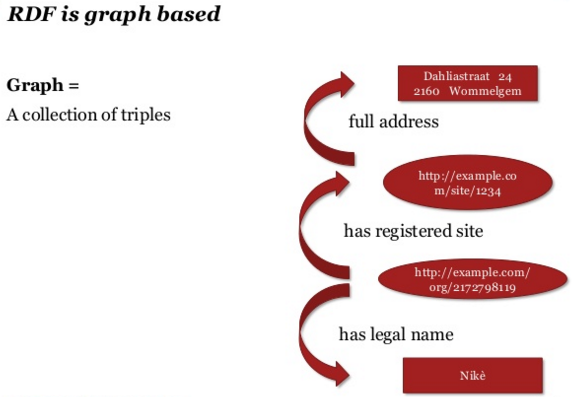
\includegraphics[height=7.5cm]{./2.PNG}
\end{frame}

%-------------------------%
\subsection{Freebase}
\begin{frame}{Freebase}
\begin{itemize}
  \item \visible<1->{Freebase is a collaborative knowledge base, which organizes data in RDF triple format  \texttt{<subject> <predicate> <object>}}

  \visible<2->{\item Subject is always a Freebase topic (equivalent to an entity)}

  \visible<3->{\item Object may be a Freebase topic or a literal value like string, booleans or numberic values}

  \visible<4->{\item Predicate is always a Freebase property (equivalent to a relation)}

  \visible<5->{\item Freebase property are grouped under Freebase types which are further grouped Freebase Domains}

  \visible<6->{\item Freebase Property Id is of the form '/domain/type/property'}

  \visible<7->{\item Multiple freebase properties may have same property names but they are used in different contexts

  \begin{itemize}

  \item Example: /music/artist/genre and /book/book/genre have same property
name but grouped under separate domain and type
  \end{itemize}}
\end{itemize}

\end{frame}

\subsection{SPARQL}
\begin{frame}{SPARQL}
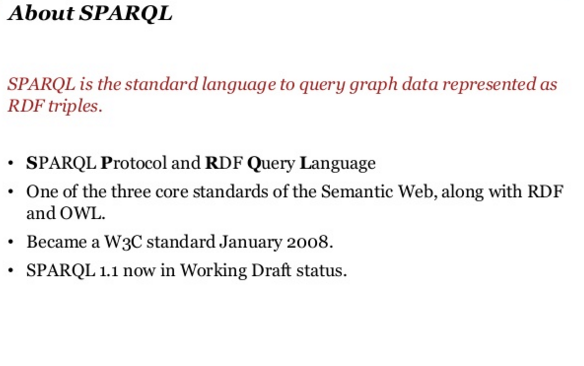
\includegraphics[height=7.5cm]{./4.PNG}
\end{frame}

\begin{frame}{SPARQL}
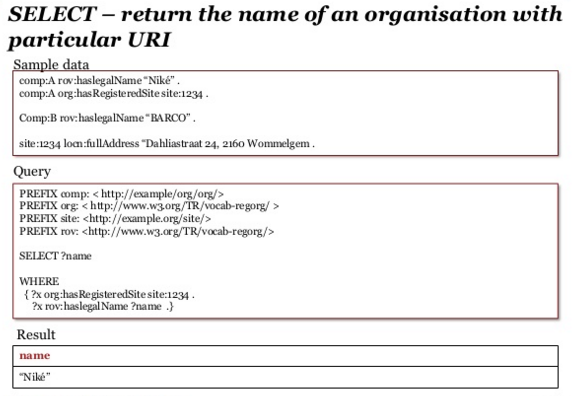
\includegraphics[height=7.5cm]{./5.PNG}
\end{frame}


%-------------------------%
\subsection[ERQ Model]{Entity Relationship Query Model}

\begin{frame}[fragile]{Entity Relationship Query Model}

\begin{itemize}
  \item Lets user specify expected entity types along with 'selection predicates' for entities and `relation predicates' between entities.
  \pause
  \item Given a query: `Find PERSON near Stanford graduate, and
COMPANY near ``Silicon Valley", where PERSON founded
COMPANY', its ERQ form is:
  \pause
  \begin{verbatim}
  SELECT x, y
FROM PERSON x, COMPANY y
WHERE x : [`Stanford', `graduate']
WHERE y : [`Silicon Valley']
AND x, y : [`found']
\end{verbatim}
  \pause
  \item \verb|`x'|, \verb|`y'| are variables bounded by types \verb|`PERSON'| and
\verb|`COMPANY'|
  \pause
  \item \verb|`Stanford', `graduate'| and \verb|`Silicon Valley'| are selection predicates
  \pause
  \item \verb|`found'| is the relation predicate between x and y
\end{itemize}

\end{frame}


%-----------------------%
\section{Related Work}

\begin{frame}
  \tableofcontents[currentsection,hideallsubsections]
\end{frame}


%-------------------------%
\begin{frame}{SPARQL translation approach}
DEANNA translates keyword queries to SPARQL queries. It involves the following steps:
\begin{itemize}
\item Phrases which can map to entities and predicates are detected.

\item Phrase to semantic mapping is done.

\item Triples of phrases are generated.

\item The query is then transformed into a SPARQL query.
\end{itemize}
\end{frame}

\begin{frame}{Querying by example entity tuples}
\begin{itemize}
\item
Since the user doesn't know what the predictes are, querying by example tuples could be used to figure out the predicates.

\item The user input and output of GQBE are both entity tuples,
called query tuples and answer tuples, respectively.

\item Say the user wants to find out "Who is the founder of Microsoft?"

\item The user could give the input as "Steve Jobs" and "Apple". Based on this the system would figure out that the predicate the user is referring to is perhaps "founded\_by".

\item Now when the user inputs "Microsoft", the system would figure out the triple corresponding to the entity "Microsoft" and predicate "founded\_by" and thus would return "Bill Gates".

\end{itemize}
\end{frame}

\begin{frame}{Interactive queries using user input}
The conceptual process of incremental query construction can be modeled as follows:
\begin{itemize}
\item
Given a database whose schema is G = (V,E), a user
issues a keyword query K = $\{$k1, k2, ..., kn$\}$.
\item The system generates all possible query interpretations of K based on G. We call this set of query interpretations $\tau$.
\item The system generates an interaction option IO and presents it to the user.
\item If the user accepts IO, then the system removes all the query interpretations that cannot imply IO from $\tau$. Otherwise, the system removes all the interpretations that imply IO from $\tau$.
\item The system retrieves the top-k query interpretations
from $\tau$, and presents them to the user.
\item If the user finds the intended query interpretation from the top-k, the query construction process terminates. Otherwise, the process generates another interaction option IO and
presents it to the user.
\end{itemize}
\end{frame}

\begin{frame}{Query interpretation based on history}
\begin{itemize}
\item
This approach uses previous queries to help during the disambiguation process. The effect that a previous query has is a combination of historical impact factor(hif) and relevance factor.

\item hif for a query done at time t on a query done a time T is:
\begin{align}
hif(t) = \frac{1}{b^{T-t}}
\end{align}

\item relevance factor indicates how relevant the previous query is to the current disambiguation. For eg if Q1 had “Ferrari, price” and Q2 had “Jaguar, speed” and an entity in Q1 was disambiguated as being a car, then the relevance factor for Jaguar "the car" will be more than Jaguar "the animal".

\end{itemize}
\end{frame}


%--------------------------%
\section[ER Keyword Querying]{Entity Relationship Keyword Queries}

\begin{frame}
  \tableofcontents[currentsection,hideallsubsections]
\end{frame}


%--------------------------%
\subsection{Query Model}


\begin{frame}{Entity Relationship Keyword Query Model}

\visible<1->{The user specifies the following:}
\begin{enumerate}
  \item<2-> n: the number of entities desired in a result
  \begin{itemize}
    \item<3-> let $e_1, e_2, ..., e_n$ denote the entity variables
  \end{itemize}
  \item<4-> $C_1, C_2, ..., C_n$: where each $C_i$ is a list of category keywords for entity variable $x_i$
  \item<5-> $K_1, K_2, ..., K_n$: where each $K_i$ is a list of selector keywords for entity variable $x_i$
  \item<6-> $R_{ij}$ for $1 \le i, j \le n$: where each $R_{ij}$ is a list of relation keywords describing the relationship between entities $x_i$ and $x_j$ $(i \ne j)$
\end{enumerate}

\end{frame}


%---------------------%
\subsection{Example Query}
\begin{frame}{An Example Query}
\visible<1->{``Find the parent-child pairs of US presidents who have attended the same university"}

\vspace{11pt}

\visible<2->{The query demands three entities $e_1$, $e_2$, and $e_3$---$e_1, e_2$ are the presidents, and $e_3$ their common alma mater.}

\vspace{11pt}


\visible<3->{Possible ER keyword query:}
\begin{itemize}
\item<4-> Number of entities is 3.
\item<5-> $C_1=$\{`person'\}, $C_2=$\{`person'\}, and $C_3=$\{`university'\}.
\item<6-> $K_1=$\{`US', `President'\}, $K_2=$\{`US', 'President'\}, and $K_3=$\{\}.
\item<7-> $R_{12}=$\{`parent'\}, $R_{13}=$\{`education'\}, and $R_{23}=$\{`education'\},
\end{itemize}

\end{frame}

%----------------------%
\subsection{Query Graph}
\begin{frame}{Query Graph}

\visible<1->{ER query can be thought of as edge-labelled directed graph $G = (V, E)$
$V = \{e_1, e_2, ..., e_n\}$ and $E = \{(e_i \xrightarrow{R_{ij}} e_j) \; | \; \forall \; R_{ij} \in \text{query} \}$.}

\visible<2->{Answering the query would then mean finding subgraphs in the data that \emph{match} the query graph. }

\vspace{11pt}

\visible<3->{ER keyword query model can be viewed as a relaxed variant of SPARQL}

\vspace{11pt}

\visible<4->{Discussion of AGGREGATE, SORT etc. queries left for future work}

\end{frame}
%---------------------%
\subsection{Query Processing}
\begin{frame}{Query Processing Overview}

\visible<1->{Keywords supplied in a user query will not in general match those used for data representation in the underlying data source. }

\vspace{11pt}

\visible<2->{To achieve superior recall, we must explore many possible \emph{meanings} of a keyword used by the user. }

\vspace{11pt}

\visible<3->{User specified keyword could be ambiguous: could could mean any of a number of entities/predicates in the data. }

\vspace{11pt}

\visible<4->{To achieve superior precision, we must be able to disambiguate the intent of the user query. }

\vspace{11pt}

\visible<5->{Our approach: ask user for help!}

\end{frame}

%-------------------------%

\begin{frame}{Query Processing Overview}

\visible<1->{Divide the problem into:}
\begin{itemize}
\item<2-> Inferring a set of candidate relation predicates, for each predicate keyword
\item<3-> Allow the user to select a subset of candidate predicates
\item<4-> Inferring a set of candidate entities, for each entity variable
\item<5-> Allow the user to select a subset of candidate entities
\item<6-> Repeat
	\end{itemize}


%\tikzstyle{int}=[draw, fill=blue!20, minimum size=2em]
%\tikzstyle{init} = [pin edge={to-,thin,black}]
% --- incomplete --- %
%\begin{tikzpicture}[node distance=5.5cm,auto,>=latex']
 %   \node [int, pin={[init]above:$v_0$}] (a) {predicate selection};
   % \node (b) [left of=a,node distance=2cm, coordinate] {a};
 %   \node [int, pin={[init]above:$p_0$}] (c) [right of=a] {entity selection};
   % \node [coordinate] (end) [right of=c, node distance=2cm]{};
   % \path[->] (b) edge node {$a$} (a);
  %  \path[->] (a) edge node {$v$} (c);
   % \draw[->] (c) edge node {$p$} (end) ;
%\end{tikzpicture}


%\tikzstyle{init} = [pin edge={to-,thin,black}]

\visible<7->{
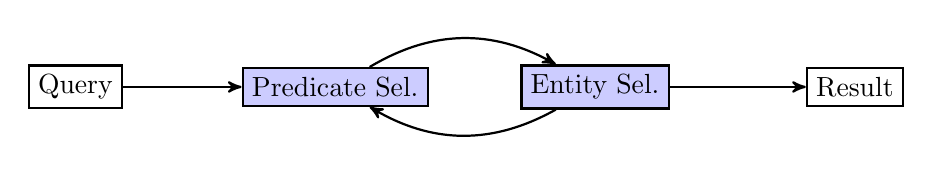
\begin{tikzpicture}[->,>=stealth',auto,node distance=3.3cm,
  thick,main node/.style={rectangle,draw, fill=blue!20},
  side node/.style={rectangle, draw}]
  \node[side node] (1) {Query};
  \node[main node] (2) [right of=1] {Predicate Sel.};
  \node[main node] (3) [right of=2] {Entity Sel.};
  \node[side node] (4) [right of=3] {Result};

  \path[every node/.style={font=\sffamily\small}]
    (1) edge node [right] {} (2)
    (2) edge [bend left] node [right] {} (3)
    (3) edge node [right] {} (4)
    (3) edge[bend left] node [left] {} (2);
%    (4) edge[bend right] node [left] {} (1);
\end{tikzpicture}
}
\end{frame}

%-------------------%

\begin{frame}{Predicate Selection for predicate $p_{ij}$}
\begin{itemize}
\item<1-> The system presents a set of candidate predicates that match the given relation keywords $R_{ij}$
\item<2-> User is expected to select of subset of these predicates that align with her intent
\end{itemize}

\vspace{11pt}

\visible<3->{To be ensured that a small enough, yet accurate enough set of candidate predicates is presented to the user, in order to minimize user effort.}

\vspace{11pt}

\visible<4->{Predicate selection for $p_{ij}$, is performed for each of the relations $x_i \sim x_j$ specified initially by the user.}

\end{frame}
%-------------------%
\begin{frame}{Entity Selection}
\visible<1->{After we have a set of valid predicates for $p_{ij}$ from the predicate selection step, try to determine the entities $x_i$ and $x_j$ obeying relation $p_{ij}$}

\vspace{11pt}

\visible<2->{The RDF graph is queried to find all entities $x_i$ and $x_j$ that match the triple pattern $\langle x_i, p, x_j \rangle$ ($p$ is one valid predicate for $p_{ij}$)}

\vspace{11pt}

\visible<3->{The set of entities (for $x_i$) is further filtered based on information from selector keywords $K_i$ and category keywords $C_i$.}

\vspace{11pt}

\visible<4->{The resulting set of entities is presented to the user (for selection) as candidate entities}

\end{frame}

%------------------%
\subsection{Query Interpretation}
\begin{frame}{Query Interpretation}
\visible<1->{Need to choose a few top predicates (entities) to be exposed to the user in the predicate (entity) selection step.}

\vspace{11pt}

\visible<2->{Need to rank predicates and entities.}

\vspace{11pt}

\visible<3->{We follow a generative approach.}

\end{frame}

%-------------------%
\begin{frame}{Predicate Selection}
\visible<1->{Let $\vec{q} = (R_{ij}, C_i, C_j, K_i, K_j)$ denote the part of the query pertaining to the predicate $p_{ij}$ and entities $x_i$, $x_j$. We are interested in $\argmax_{p}$Pr$(p|\vec{q})$, where}


\begin{align*}
\visible<2->{\text{Pr}(p|\vec{q}) &\propto \text{Pr}(p, \vec{q}) = \text{Pr}(p)\cdot \text{Pr}(\vec{q}|p) = \text{Pr}(p)\cdot \sum_{t_{i}, t_{j}} \text{Pr}(\vec{q}, t_i, t_j | p)} \\
\visible<3->{&= \text{Pr}(p)\cdot \sum_{t_{i}, t_{j}} \text{Pr}(R_{ij}, C_i, C_j, K_i, K_j, t_i, t_j| p)} \\
\visible<4->{&= \text{Pr}(p)\cdot \sum_{t_{i}, t_{j}} \text{Pr}(R_{ij}|p)\cdot\underbrace{\text{Pr}(t_i,t_j|R_{ij},p)}_\text{(I)}\cdot\underbrace{\text{Pr}(C_i,C_j|t_i,t_j,R_{ij},p)}_\text{(II)}\cdot \phi_1}
\end{align*}


\visible<5->{where $\phi_1$ is defined as:}
\begin{align*}
\visible<6->{\phi_1(K_i,K_j,C_i,C_j,e_i,e_j,t_i,t_j,R_{ij},p) = \text{Pr}(K_i,K_j|C_i,C_j,e_i,e_j,t_i,t_j,R_{ij},p) }
\end{align*}

\end{frame}


%-------------------%
\begin{frame}{Simplifying the math}
\visible<1->{Make reasonable independence assumptions:}

\begin{enumerate}
\item<2-> $\text{Pr}(t_i,t_j|R_{ij},p) = \text{Pr}(t_i,t_j|p)$

\item<3-> $\text{Pr}(C_i,C_j|t_i,t_j,R_{ij},p) = \text{Pr}(C_i,C_j|t_i,t_j)$

\item<4-> $\text{Pr}(C_i,C_j|t_i,t_j) = \text{Pr}(C_i|t_i) \cdot \text{Pr}(C_j|t_j)$
\end{enumerate}


\end{frame}

%------------------%
\begin{frame}{More latent variables}

\visible<1->{By introducing the latent variables $e_i$ and $e_j$ for entities represented by $x_i$ and $x_j$ in the query, we can rewrite $\phi_1$ as:}

\begin{align*}
\visible<2->{\phi_1 &= \text{Pr}(K_i,K_j|C_i,C_j,t_i, t_j,R_{ij},p) = \sum_{e_i,e_j}\text{Pr}(K_i,K_j,e_i,e_j|C_i,C_j,t_i,t_j,R_{ij},p)} \\
\visible<3->{&= \sum_{e_i,e_j} \text{Pr}(e_i,e_j|C_i,C_j,t_i,t_j,R_{ij},p) \cdot \text{Pr}(K_i,K_j|e_i,e_j,C_i,C_j,t_i,t_j,R_{ij},p)}
\end{align*}

\end{frame}

%-------------------%

\begin{frame}{More independence assumptions}

\visible<1->Assume:
\begin{enumerate}
\item<2-> $\text{Pr}(e_i,e_j|C_i,C_j,t_i,t_j,R_{ij},p) = \text{Pr}(e_j,e_j|t_i,t_j,p)$

\item<3-> $\text{Pr}(K_i,K_j|e_i,e_j,C_i,C_j,t_i,t_j,R_{ij},p) = \text{Pr}(K_i,K_j|e_i,e_j)$

\item<4-> $\text{Pr}(K_i,K_j|e_i,e_j) = \text{Pr}(K_i|e_i)\cdot \text{Pr}(K_j|e_j)$
\end{enumerate}
\end{frame}

%-------------------%

\begin{frame}{Finally}
\visible<1->{Finally we have:}

\begin{align*}
\visible<2->{\text{Pr}(p|\vec{q})& \propto \text{Pr}(p) \cdot \sum_{t_i,t_j,e_i,e_j} \phi_2(p, R_{ij}, C_i, C_j, K_i, K_j, t_i, t_j, e_i, e_j)}
\end{align*}

\visible<3->{where $\phi_2$ is defined as,}


\begin{align*}
\visible<4->{\phi_2 = \text{Pr}(R_{ij}|p) & \cdot \text{Pr}(t_i,t_j|p) \cdot \text{Pr}(C_i|t_i) \cdot \text{Pr}(C_j|t_j)} \\
\visible<4->{& \cdot \text{Pr}(e_i,e_j|t_i,t_j,p) \cdot \text{Pr}(K_i|e_i) \cdot \text{Pr}(K_j|e_j)}
\end{align*}


\end{frame}


%------------------%
\begin{frame}{Estimating $\text{Pr}(p)$}

\visible<1->{$\text{Pr}(p)$ is simply the prior on the predicate $p$. We estimate it as:}
\visible<2->{$$\text{Pr}(p) = \frac{\text{freq}(p)}{\sum_{p_i \in \mathbb{P}}\text{freq}(p_i)}$$}

\visible<3->{where $\mathbb{P}$ is the set of all possible predicates in our RDF data source.}
\end{frame}


%------------------%
\begin{frame}{Estimating $\text{Pr}(R_{ij}| p)$, $\text{Pr}(C_i| t_i)$, $\text{Pr}(K_i| e_i)$}

\visible<1->{Let us start with $\text{Pr}(R_{ij}| p)$}

\vspace{11pt}

\visible<2->{Use an entity-annotated corpus for discovering phrase patterns for predicate $p$}

\visible<3->{E.g. ClueWeb09 corpus annotated with Freebase entities}


\begin{enumerate}
\visible<4->{\item For each predicate $p$, consider all triples and locate all the corpus sentences that mention both the participating entities of the triple.}
\visible<5->{\item If the entities $e_i$ and $e_j$ co-occur in a sentence then this sentence is an evidence of the triple $\langle e_i, p, e_j \rangle$}
\visible<6->{\item Using MaltParser obtain dependency graph for each sentence}
\visible<7->{\item Words in the path connecting the entities are joined together and added to a candidate phrase dictionary, provided the path is at most 3 hops}

\end{enumerate}

\end{frame}

%-------------------%
\begin{frame}{Estimating $\text{Pr}(R_{ij}| p)$}

\visible<1->{Thus, we have, for all predicates $p$, a list $\mathbb{R}_{ij}$ of all phrases that are known to hint at $p$.}
\visible<2->{We can then estimate $\text{Pr}(R_{ij}| p)$ as:}

\begin{align*}
\visible<3->{\text{Pr}(R_{ij}| p) = \frac{n(p, R_{ij})}{\sum_{R'_{ij} \in \mathbb{R}_{ij}}{n(p, R'_{ij})}}}
\end{align*}
 \visible<4->{where $n(p, R_{ij})$ represents the number of sentences in which $R_{ij}$ occurred as a phrase in the dependency path between entities participating in relation specified by predicate $p$.}
\end{frame}

%--------------------%
\begin{frame}{Estimating $\text{Pr}(t_i,t_j|p)$}
\visible<1->{For predicate $p$, we all the triples that it is involved in, and filter those out  in which the connected subject and object have types $t_i$ and $t_j$ respectively. Let $n(p; t_i, t_j)$ be the number of such triples. Then, simply}

\begin{align*}
\visible<2->{\text{Pr}(t_i,t_j|p) = \frac{n(p; t_i, t_j)}{n(p)}}
\end{align*}
\visible<3->{where $n(p)$ denotes the number of triples in Freebase that have $p$ as the predicate.}

\visible<4->{Note that the filtering operation above can be easily carried out in case of Freebase due to the availability of a \texttt{/object/type/} relation for most entities.}

\end{frame}


%----------------------%

\begin{frame}{Estimating $\text{Pr}(e_i,e_j|t_i,t_j,p)$}

\visible<1->{Though $\text{Pr}(e_i,e_j | t_i,t_j,p)$ must take into account the $e_i$--$t_i$, and $e_j$--$t_j$ compatibility, we make a simplifying assumption without deviating a lot from the intended semantics of $\text{Pr}(e_i,e_j|t_i,t_j,p)$.}

\visible<2->{Define,}
\begin{align*}
\visible<2->{\text{Pr}(e_i,e_j | t_i,t_j,p) = \frac{n(e_i, e_j; p)}{n(p)} }
\end{align*}

\visible<3->{where $n(e_i, e_j; p) = 1$ if the triple $\langle e_i, p, e_j \rangle$ occurs in the data, otherwise $n(e_i, e_j; p) = 0$.}

\visible<4->{As earlier, $n(p)$ denotes the number of triples that have $p$ as their predicate part.}

\end{frame}

%----------------------%

\begin{frame}{Computation}

\visible<1->{We started off with computing}
\begin{multline*}
\visible<2->{\text{Pr}(p) \cdot \sum_{t_i,t_j,e_i,e_j}  \text{Pr}(R_{ij}|p) \cdot \text{Pr}(t_i,t_j|p) \cdot \text{Pr}(C_i|t_i) \cdot \text{Pr}(C_j|t_j)} \\
 \visible<2->{\cdot \text{Pr}(e_i,e_j|t_i,t_j,p) \cdot \text{Pr}(K_i|e_i) \cdot \text{Pr}(K_j|e_j) }
\end{multline*}

\visible<3->{Note that only $\text{Pr}(e_i, e_j | t_i, t_j, p)$ involves all the summation variables $t_i, t_i, e_i, e_i$ and can be expensive to compute. The summation on the other terms can be computed rather cheaply.}

\vspace{11pt}

\visible<4->{Simply set $\text{Pr}(e_i, e_j | t_i, t_j, p) = 1$. }


\visible<5->{The burden of producing a valid \emph{score} rests divided on all the $\text{Pr}$'s involved, and we expect that the results will not be perturbed much on ignoring one of the $\text{Pr}$'s.}


\end{frame}

%----------------------%
\begin{frame}{Score computation}

\visible<1->{The argmax computation that we started off initially with can be replaced by a \emph{score} computation for each of the predicates. }

\vspace{11pt}

\visible<2->{On cleaning our Freebase dataset we ended up with only 6200 distinct predicates}

\vspace{11pt}

\visible<3->{The score computation will be generally feasible, given that several of the quantities can be precomputed and stored.}
\end{frame}

%-----------------------%
\begin{frame}{Entity Selection}

\visible<1->{Let $e$ denote a candidate entity (unknown) for the entity variable $e_i$ and let $\vec{q_{e_i}} = (K_i, C_i)$ be the part of the query pertaining directly to $e_i$. As before, we are interested in $\argmax_{e} \text{Pr}(e|\vec{q_{e_i}})$, where}


\begin{align*}
\visible<2->{\text{Pr}(e|\vec{q_{e_i}}) \propto \text{Pr}(e, \vec{q_{e_i}}) & = \text{Pr}(e) \cdot \text{Pr}(\vec{q_{e_i}}|e)}  \\
\visible<3->{ &= \text{Pr}(e) \cdot \sum_{p_{ij_1}, p_{ij_2},..., p_{ij_r}}\text{Pr}(\vec{q_{e_i}}, p_{ij_1}, p_{ij_2},..., p_{ij_r} | e)} \\
\visible<4->{&= \text{Pr}(e) \cdot \sum_{p_{ij_1}, p_{ij_2},..., p_{ij_r}}\text{Pr}(K_i, C_i, p_{ij_1}, p_{ij_2},..., p_{ij_r} | e)}
\end{align*}

 \begin{align*}
\visible<5->{  = \text{Pr}(e) \cdot \sum_{p_{ij_1}, p_{ij_2},..., p_{ij_r}} \text{Pr}(K_i | e) \cdot \text{Pr}(C_i | K_i, e) \cdot \text{Pr}(p_{ij_1}, p_{ij_2},..., p_{ij_r} | C_i, K_i, e) }
\end{align*}


\end{frame}

\begin{frame}{Entity Selection}

\visible<1->{The summation in the last slide is obtained by the introduction of latent variables $p_{ij_1}, p_{ij_2},..., p_{ij_r}$, that denote the various predicates that are on the outgoing edges from $e_i$ in the query graph.}

\vspace{11pt}

\visible<2->{We arrive at the entity selection stage only after one or more stages of predicate selection.}

\visible<3->{The variables $p_{ij_1}, p_{ij_2},..., p_{ij_r}$ range over $\mathbb{P}_{ij_1}, \mathbb{P}_{ij_2}, ...,\mathbb{P}_{ij_r}$ respectively, where $\mathbb{P}_{ij_k} (1 \le k \le r)$ denote the set of selected candidate predicates in previous predicate selection stage(s). $\mathbb{P}_{ij_k} = \emptyset$, in case predicate selection stage has not occurred for $p_{ij_k}$, yet.}

\end{frame}

%-------------------------%
\begin{frame}{Simplifying the math}
\visible<1->{Independence assumptions:}
\begin{enumerate}
\item<2-> $\text{Pr}(C_i|K_i,e) = \text{Pr}(C_i|e)$
\item<3-> $\text{Pr}(p_{ij_1}, p_{ij_2},..., p_{ij_r} | C_i, K_i, e) = \prod_{k=1}^{r} \text{Pr}(p_{ij_k} | e)$
\end{enumerate}

\vspace{11pt}
\visible<4->{Equation is reduced to:}
\begin{align*}
\visible<5->{\text{Pr}(e, \vec{q_{e_i}}) &= \text{Pr}(e) \cdot \text{Pr}(K_i | e) \cdot \text{Pr}(C_i | e) \cdot \sum_{p_{ij_1}, p_{ij_2},..., p_{ij_r}}  \prod_{k=1}^{r} \text{Pr}(p_{ij_k} | e) }
\end{align*}

\end{frame}

%-------------------------%
\begin{frame}{Estimating $\text{Pr}(e)$}

\visible<1->{$\text{Pr}(e)$ is simply the prior on entity $e$. We estimate it as:}
\visible<2->{$$\text{Pr}(e) \approx \frac{\text{freq}(e)}{\sum_{e_i \in \mathbb{E}}\text{freq}(e_i)}$$}
\visible<3->{where $\mathbb{E}$ is the set of entities considered for ranking.}

\end{frame}

%-------------------------%
\begin{frame}{Estimating $\text{Pr}(K_i| e)$}

An initial approach is to use WordNet synsets of the short description available for the entity $e$; and set $\text{Pr}(K_i| e)$ for any matching words in the synsets.
\end{frame}


%-------------------------%
\begin{frame}{Estimating $\text{Pr}(C_i| e)$}

\visible<1->{A Freebase entity can in general, be associated with several types $t_1, ..., t_m$. We define, }
\begin{align*}
\visible<2->{ \text{Pr}(C_i| e) = \sum_{j=1}^{m} \text{Pr}(C_i| t_j)}
\end{align*}
\visible<3->{where $\text{Pr}(C_i| t_j)$ can be used as discussed for predicate in the previous section.}

\end{frame}


%-------------------------%
\begin{frame}{Estimating $\text{Pr}(p_{ij_{k}}| e)$}

\visible<1->{It is natural to have the following definition,}
\begin{align*}
\visible<2->{\text{Pr}(p_{ij_{k}}| e) = \frac{n(p_{ij_{k}}, e)}{n(e)}}
\end{align*}
\visible<3->{where $n(p_{ij_{k}}, e)$ is the number of triples that have $e$ related by the predicate $p_{ij_{k}}$, and $n(e)$ is the total number of triples of $e$.}


\end{frame}

%-------------------------%
\begin{frame}{Computation}

\visible<1->{The original equation, when rewritten in product-of-sum form, is not expected to be computationally expensive owing to the following observations: }
\begin{enumerate}
  \item<2-> The predicates $p_{ij_1}, p_{ij_r}, ..., p_{ij_r}$ are the predicates that are labels of outgoing edges of entity variable $e_i$ in the query graph. Therefore, for even the most convoluted (and meaningful) queries one can think of, $r$ would be a small number ($< 10$ let's say).
  \item<3-> The predicate selection step would have been completed for these predicates before entity selection is done for the entity variable $e$. This limits the total number of terms in the sum, allowing for cheap computation of the overall \emph{score}.
\end{enumerate}


\begin{itemize}
\item<4-> Do not do scoring for all entities!
\item<5-> Perform a keyword search using the selector keywords (and their synonyms) of the entity and to perform ranking for the result entities
\end{itemize}

\end{frame}

%-------------------------%
\begin{frame}{Result of the query}


\visible<1->{At this stage, we have a set of selected entities for each entity variable sought by the query, and also a set of selected predicates for each of the relations between pairs entity variables in the query.}

\vspace{11pt}

\visible<2->{Compute the join of selected entity set of $e_i$ with those of its immediate neighbors in the query graph.}

\vspace{11pt}
\visible<3->{Further filtering may be required to discard (entity-predicate-entity) tuples that do not have matching triples in the data.}


\end{frame}


%-------------------------%
\section{Conclusion}
\begin{frame}{Conclusion}
\begin{itemize}
\item<1-> The Entity Relationship Keyword Querying framework, provides a powerful combination of ease-of-use and capability of processing complicated queries

\end{itemize}
\end{frame}


%-------------------------%
\begin{frame}[plain,c]

\begin{center}
\Huge Thank you for listening!
\end{center}

\end{frame}


\end{document}
